\documentclass[11pt]{article}
\usepackage{../../timestamp}
\usepackage{../../astro207}
\usepackage{../../markup}
\usepackage{../../fa21}
\usepackage{tikz}
\usetikzlibrary{calc,shapes.geometric,arrows,automata}
\usepackage{color,hyperref,listings,enumitem}
\usepackage{algorithm}
\usepackage{algpseudocode}
\usepackage{tkz-euclide}
\usepackage{pgfplots}
\usepackage{subcaption}
\usepackage{pdfpages}
\usepackage{bm}
\usepackage[american,siunitx]{circuitikz}
\lstset{basicstyle=\ttfamily}
\newcommand{\fillin}[1]{\underline{\hskip #1}}
\newcommand{\doublehrule}{\hrule \vskip 0.02in \hrule}
\newcommand*\circled[1]{\tikz[baseline=(char.base)]{
  \node[shape=circle,draw,inner sep=2pt] (char) {#1};}}
\usepackage{hyperref}
\hypersetup{
	colorlinks=true,
	linkcolor=black,
	urlcolor=blue
}

\begin{document}

\def\title{Problem Set 9}
% \config{hwnum}{1}
% \config{homework-due}{08/31/2018 23:59}
% \config{grades-due}{09/04/2018 23:59}

\newcommand{\qitem}{\qpart\item}

\renewcommand{\labelenumi}{(\arabic{enumi})} % change default enum format to (1)
\renewcommand{\theenumi}{(\arabic{enumi})} % fix reference format accordingly.
\renewcommand{\labelenumii}{\roman{enumii}.} % second level labels.
\renewcommand{\theenumii}{\roman{enumii}.}

\maketitle

\begin{qunlist}
\qns{A Compton Monte Carlo}

\begin{enumerate}

\qitem{\textcolor{white}{blep}}
\ans{
	\begin{figure}[H]
		\centering
		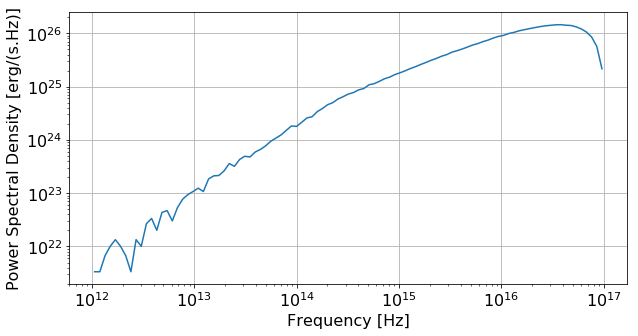
\includegraphics[width=0.8\textwidth]{./questions/q_a_compton_monte_carlo_figs/single}
		\caption{The simulated power spectral density of a single electron with $\gamma = 10$, generated via Monte Carlo sampling of uniformly distributed $\cos\theta_\text{in}$ and $\cos\theta_\text{out}'$. The cutoff (around x-ray frequencies) doesn't seem terribly unreasonable and corresponds to a few hundred eV.}
	\end{figure}
}

\qitem{}
\work{
	\begin{align*}
	    \frac{dP}{d\nu} &= \frac{dP}{d\gamma} \cdot \frac{d\gamma}{d\nu}
	\end{align*}
	\begin{multicols}{2}
		\raggedcolumns
		\begin{align*}
		    \nu &= \nu_\text{in}\gamma^2(1-\beta\cos\theta_\text{in})(1+\beta\cos\theta_\text{out}')\\
		        &\approx \nu_\text{in}\gamma^2\\
		    \frac{d\gamma}{d\nu} &\approx \frac{1}{2\sqrt{\nu_\text{in}}}\nu^{-\frac{1}{2}}
		\end{align*}
		\vfill\columnbreak
		\begin{align*}
	    \frac{dP}{d\gamma} &= \frac{dN_\gamma}{d\gamma} \cdot P\rvert_\text{single photon}\\
	        &= N_pA\gamma^{-p} \cdot L_p\gamma^2(1-\beta\cos\theta_\text{in})(1+\beta\cos\theta_\text{out}')(1-e^{-\tau})\\
	        &\approx N_pA\gamma^{-p} \cdot L_p \gamma^2(1-e^{-\tau})\\
	        &= N_pL_pA(1-e^{-\tau})\gamma^{2-p}\\
	        &\approx N_pL_pA(1-e^{-\tau})\left(\frac{\nu}{\nu_\text{in}}\right)^{1-\frac{p}{2}}
	\end{align*}
	where 
	$$A = \frac{1-p}{(\gamma_\text{max})^{1-p} - (\gamma_\text{min})^{1-p}}$$
	to enforce
	$$\int_{\gamma_\text{min}}^{\gamma_\text{max}}Ax^{-p}dx = 1$$
	\end{multicols}
	When push comes to shove,
	\begin{align*}
		\frac{dP}{d\nu} &\propto \nu^{\frac{1-p}{2}}
	\end{align*}
	over values of $\nu \in [\nu_\text{in}(\gamma_\text{min})^2, \nu_\text{in}(\gamma_\text{max})^2]$ (roughly). The plot below includes the various constants.}
\ans{
	\begin{figure}[H]
		\centering
		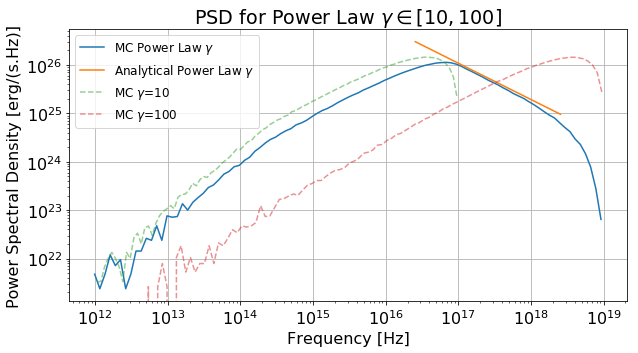
\includegraphics[width=0.8\textwidth]{./questions/q_a_compton_monte_carlo_figs/ensemble_power}
		\caption{The simulated power spectral density of an ensemble of electrons with a power law distribution of $\gamma$, i.e. $dN_\gamma = A\gamma^{-p}d\gamma$ when $\gamma_\text{min}\leq\gamma\leq\gamma_\text{max}$. The PSDs for constant, single-valued $\gamma$ at the bounds $\gamma_\text{min}$ and $\gamma_\text{max}$ are included to sanity check the behavior of the Monte Carlo simulated result past the bounds of their respective cutoff frequencies.}
	\end{figure}}
\end{enumerate}

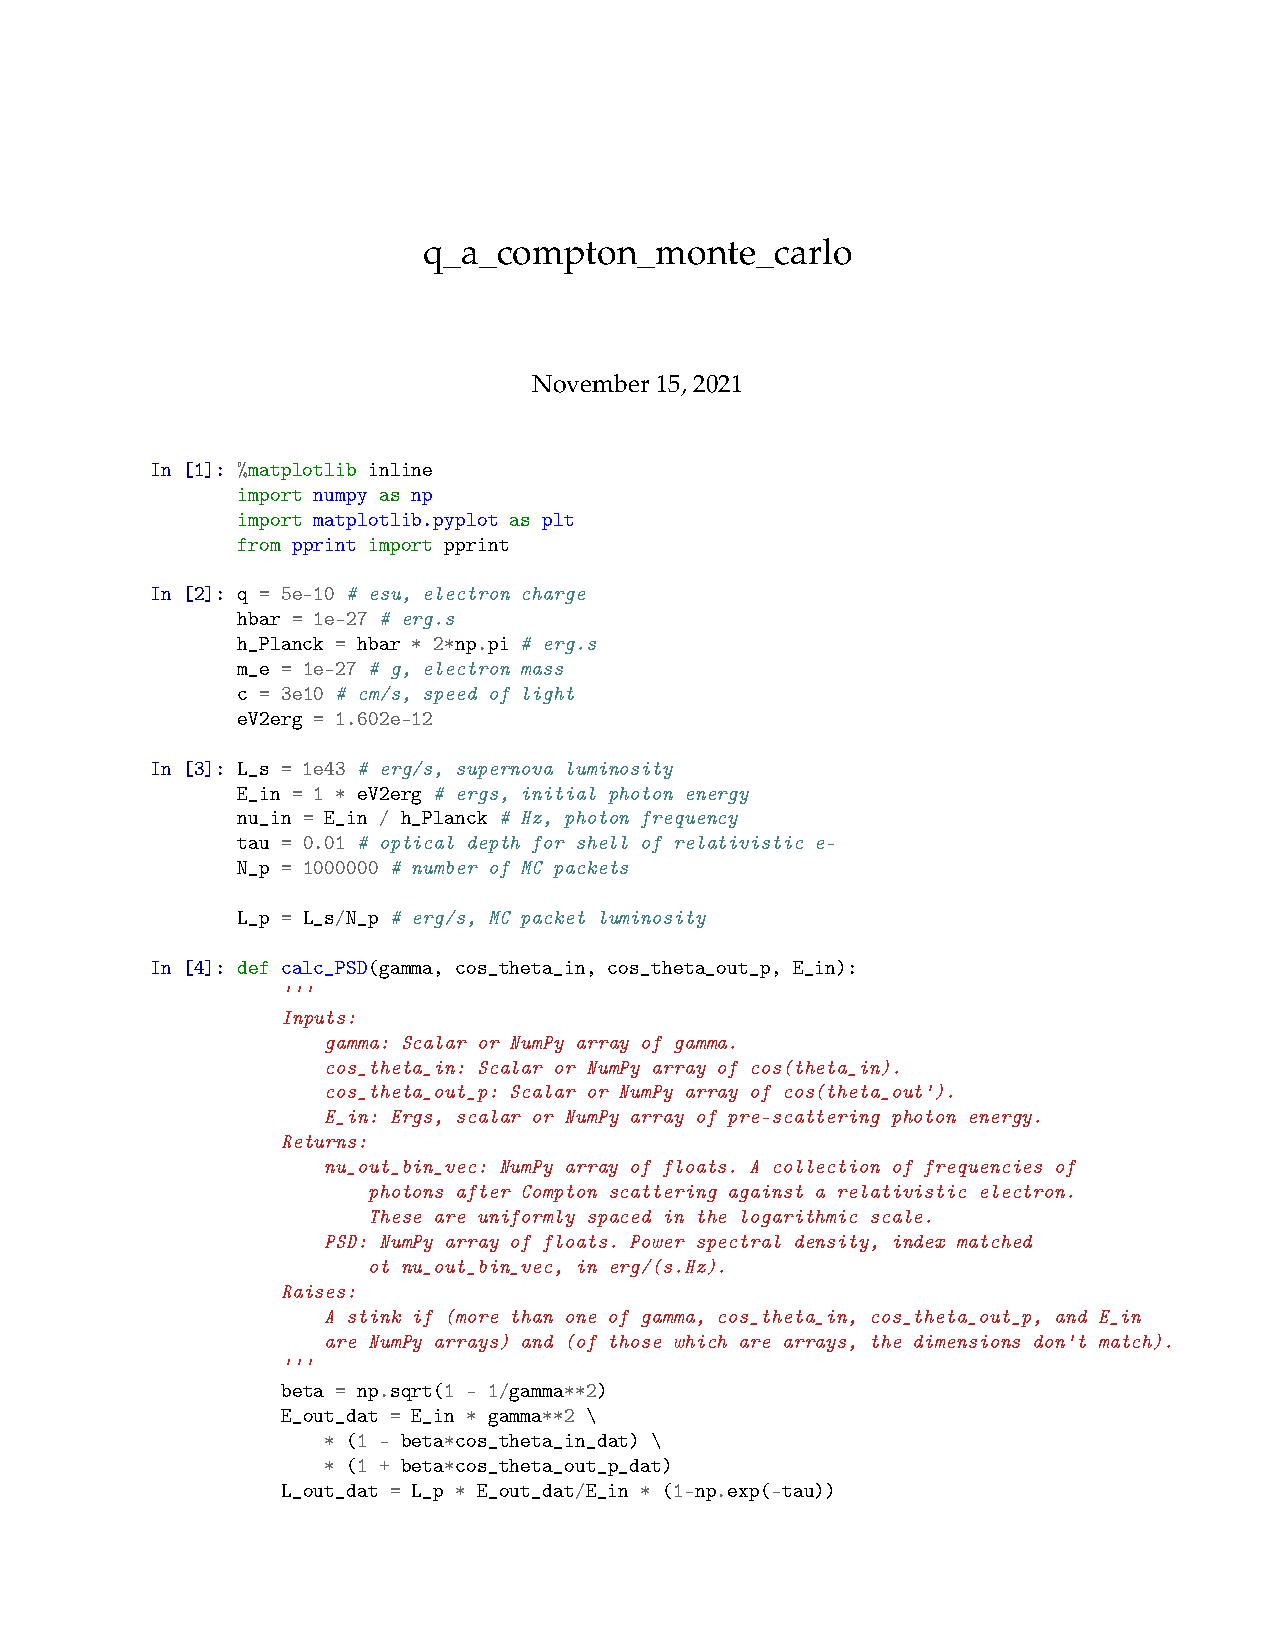
\includepdf[pages=-,offset=-2ex -10ex]{./questions/q_a_compton_monte_carlo_figs/q_a_compton_monte_carlo_ipynb.pdf}
\end{qunlist}
\end{document}
